\documentclass[a4paper,11pt]{article}
% !TeX spellcheck = en_GB
\usepackage{floatrow}
\usepackage{graphicx}
\usepackage{caption}
\usepackage{subcaption}
\usepackage{enumitem}
\usepackage{array}
\usepackage{amsmath,amssymb}
\usepackage{hyperref}
\usepackage[utf8]{inputenc}
\usepackage[T1]{fontenc}
\usepackage[margin=1.3cm]{geometry}
\usepackage{fancyvrb}
\usepackage{float}
\usepackage{wrapfig}
\usepackage[export]{adjustbox}
\usepackage{xcolor}
\usepackage{listings}
\usepackage{gensymb}
\usepackage{minted}

\title{\textbf{Final Report (Group 10)\protect\\Modeling and Verification of Digital Systems}}
\author{Eoin Brereton Hurley and Ieva Petrulionyte}
\date{}

\begin{document}
	\maketitle
    
    \section{Introduction}
    \subsection{Garage Door Controller}
    \par In this project we attempt to model part of the hardware needed to control a garage door. We focus on designing the main controller circuit which will potentially be connected to other hardware components in the system and will dictate how the system behaves in possible use scenarios. We design the controller as an abstract finite state machine and later perform two different syntheses to generate \texttt{ASIC} and \texttt{FPGA} circuits with physical components (logical gates and memory components). We also use different verification techniques such as temporal assertions, coverage analysis and simulations of different use cases to verify the behaviour of the circuit before and after synthesis.
    
    \subsection{Design Flow Description}
    \par In this project we design and synthesize a circuit that controls a garage door and allows the user to interact with the door. We start from a text specification and go through multiple design and verification phases to synthesize an \texttt{ASIC} and an \texttt{FPGA} description.
    
    \begin{figure}[H]
      \centering
      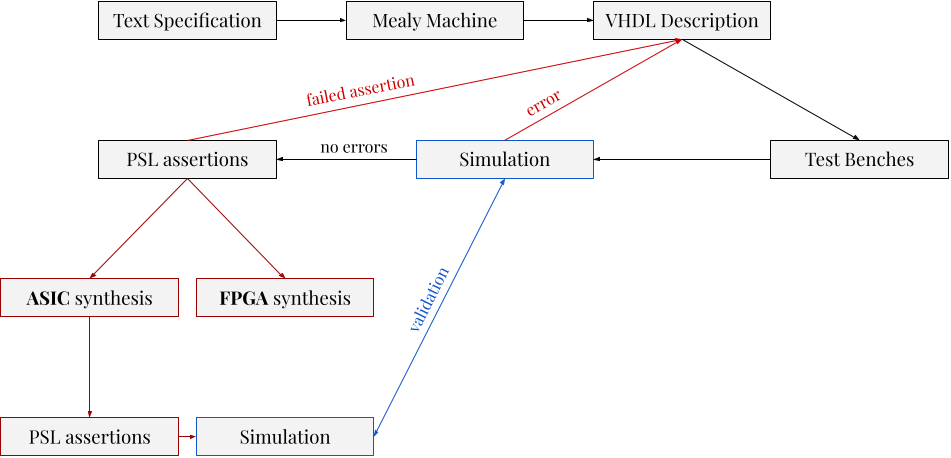
\includegraphics[width=0.8\linewidth]{design_flow.png}  
      \caption{Design Flow}
    \end{figure}
    
    \par The figure shows the design flow we follow throughout the project. From the given specification we complete a Mealy machine where the values of the outputs depend on both the current state and the values of the current inputs.
    
    \begin{figure}[H]
      \centering
      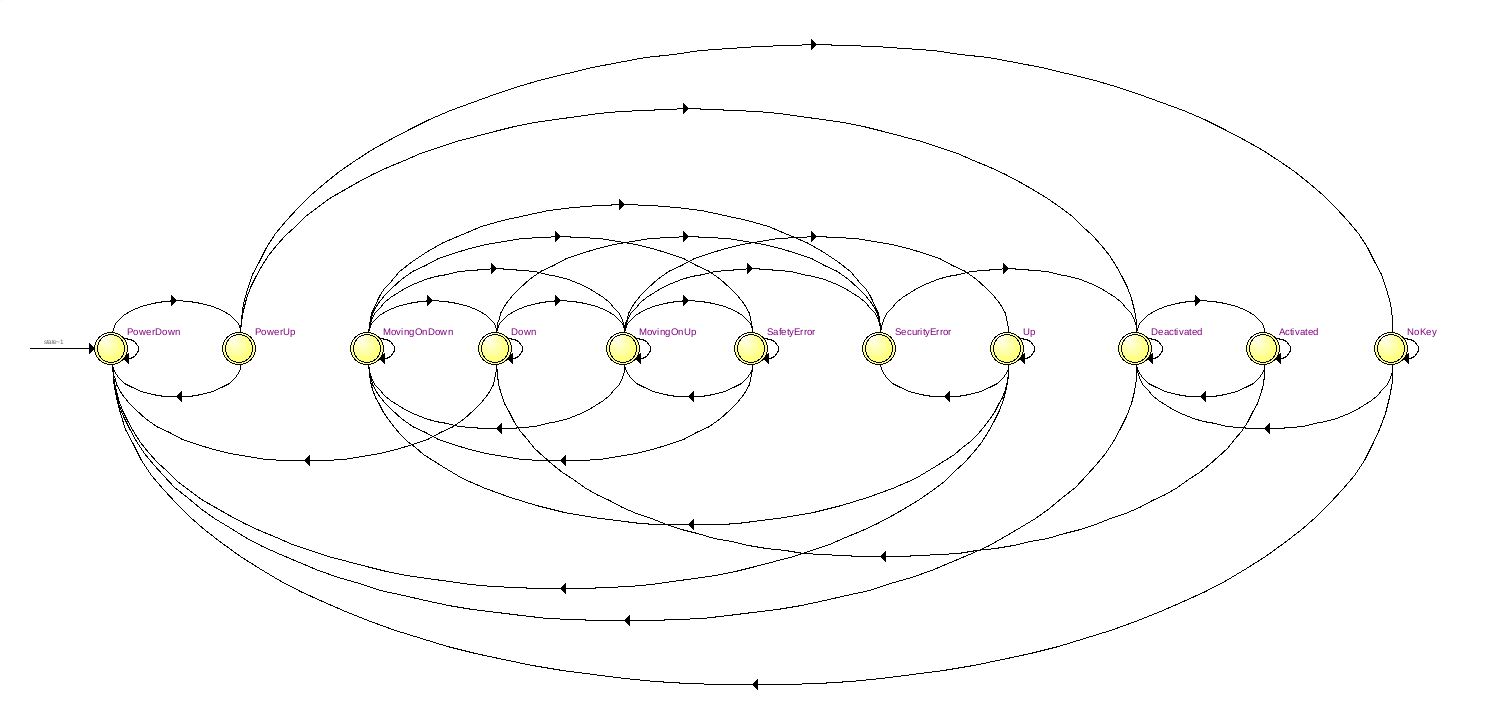
\includegraphics[width=1\linewidth]{PROJECT0_2.png}  
      \caption{Finite State Machine}
    \end{figure}
    
    \par Then, based on the completed finite-state automaton, we write the \texttt{VHDL} description of our component which consists of \textbf{3 main processes}:
    \begin{enumerate}
        \item \textbf{transition function} where the next state is decided based on current inputs and the current state, therefore this process is sensitive to all inputs and the internal state signal;
        \item \textbf{output function} where the current value of the outputs is decided based on current inputs and the current state, therefore this process is sensitive to all inputs and the internal state signal;
        \item \textbf{state update function} where the current state is updated on every clock rising edge or on a reset signal, therefore this process is sensitive to the clock and reset inputs.
    \end{enumerate}
    
	\section{Simulations}
	
	We have two main test benches with two different scenarios that we use for simulations of different use cases and validation of \texttt{PSL} assertions about the behaviour of our circuit. The code of all test benches can be found in the appendix.
	
	\subsection{Safety Error}
	
	\par This test bench covers a scenario where a user approaches the door which is initially closed and presses the controller which transmits an authentication encryption key: the key LED lights up. The key is identified as valid, the gate is activated and the authentication LED lights up. The user presses the open button, the open LED flashes and the door begins to open. While the door is opening, the user presses the close button. The close LED lights up and the door begins to close. While the door is closing, a small child runs under the door. The door stops moving. The child moves out from under the door. The door resumes closing until it is fully closed. Moments later, another user switches off the entire system.
    
    \begin{figure}[H]
      \centering
      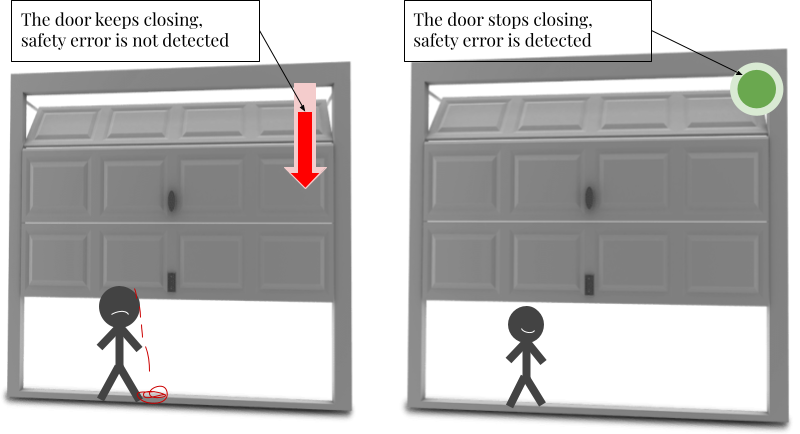
\includegraphics[width=0.55\linewidth]{scenario1_maan.png}  
      \caption{We want to avoid the situation on the left by validating the Safety Error test bench}
    \end{figure}
    
    \begin{figure}[H]
      \centering
      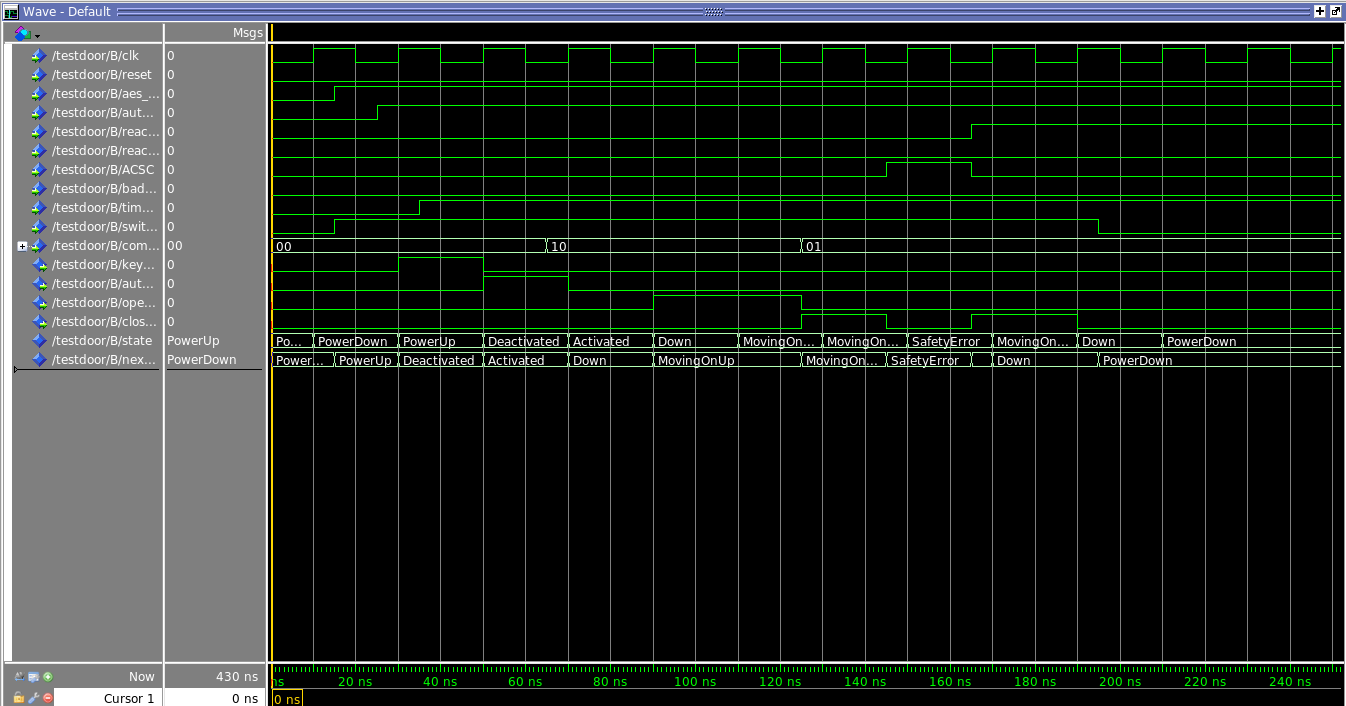
\includegraphics[width=0.9\linewidth]{scenarioSafety.png}  
      \caption{Wave form of simulating the Safety Error test bench with a 50 MHz clock}
    \end{figure}
	
	\par In the simulation waveform, we expect that when the safety error is detected (\texttt{acsc <= '1'} at \texttt{145ns}), the door which is in the process of closing will stop moving. Which is what happens since the state goes to "Safety error" on the next clock rising edge at \texttt{150ns}. We also expect the door to only start closing again when the safety threat has passed, which is the case at \texttt{165ns}.
	
	\subsection{Security Error}
	
	\par This test bench covers a scenario where the system was switched off while the door was open. The system is turned on again. A user presses the controller which transmits an authentication encryption key: the key LED lights up. The user presses the close button and subsequently the door begins to close. The user presses the close button again, but some of the signal is lost and this results in an encryption error which makes the door stop closing. The user presses the button again and this time the signal is authenticated. By validating this test we want to make sure that we avoid situations when an adversary, not the owner, tries to open the door and enter the garages by sending an unauthenticated command to the controller.
	\newline
	\par In the simulation waveform, we expect that when the security error is detected (\texttt{bad\_encryption <= '1'} at \texttt{105ns}), the door which is in the process of closing will stop moving. This is in fact the observed behaviour since the state goes to "Security error" on the next clock rising edge at \texttt{110ns}.
    
    \begin{figure}[H]
      \centering
      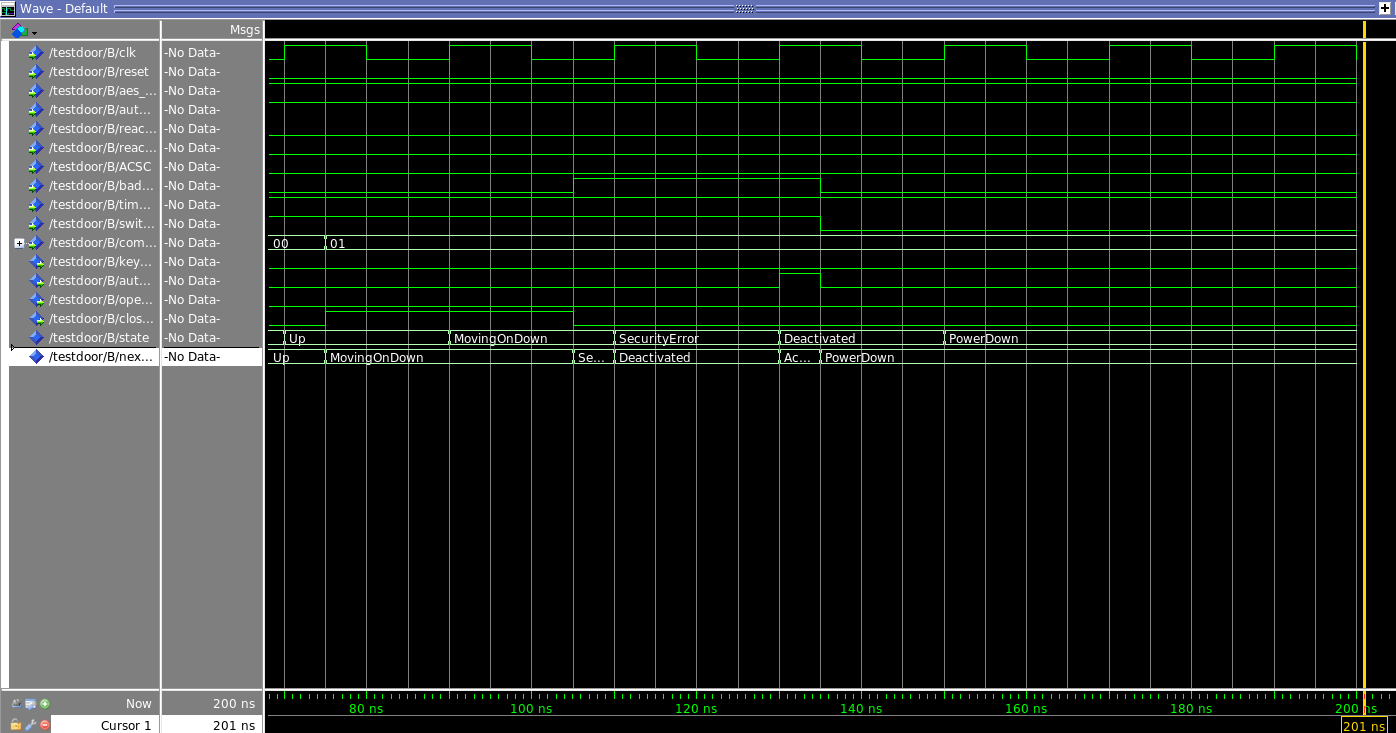
\includegraphics[width=0.9\linewidth]{scenarioSecurity.png}  
      \caption{Wave form of simulating the Security Error test bench with a 50 MHz clock}
    \end{figure}
    
    \subsection{Coverage}
	\par To get better coverage we merge the two described test benches with other smaller ones that test functionalities of opening/closing the door as well as turning on/switching off the system. The global state coverage of our tests is \texttt{100\%} and the transition coverage is \texttt{68\%}, which is acceptable knowing that all transitions from all states to the reset state are not taken into account in our test benches.
	
	\begin{minted}[mathescape]{vhdl}
=================================================================================
=== File: model.vhd
=================================================================================
    Enabled Coverage            Active      Hits    Misses % Covered
    ----------------            ------      ----    ------ ---------
    Stmts                           49        44         5      89.7
    Branches                        63        57         6      90.4
    FSMs                                                        84.0
        States                      11        11         0     100.0
        Transitions                 47        32        15      68.0
	\end{minted}
    
    \section{Validation}
    
    \subsection{\texttt{PSL} assertions}
    \subsubsection{Key required}
    We test the first \texttt{PSL} assertion \textit{key\_req} using the Safety error test bench. This assertion specifies that when the system reaches either the state  \textit{PowerUp} or  \textit{PowerDown}, it will not be able to reach the state \textit{Activated} until the encryption key has been entered. The waveform below shows that this assertion (first one out of the three that appear at the top) is validated. The correct encryption key \texttt{ak} is received at \texttt{55ns}, and subsequently a green triangle appears at the next clock rising edge showing that the assertion has passed.
    
    \begin{figure}[H]
      \centering
      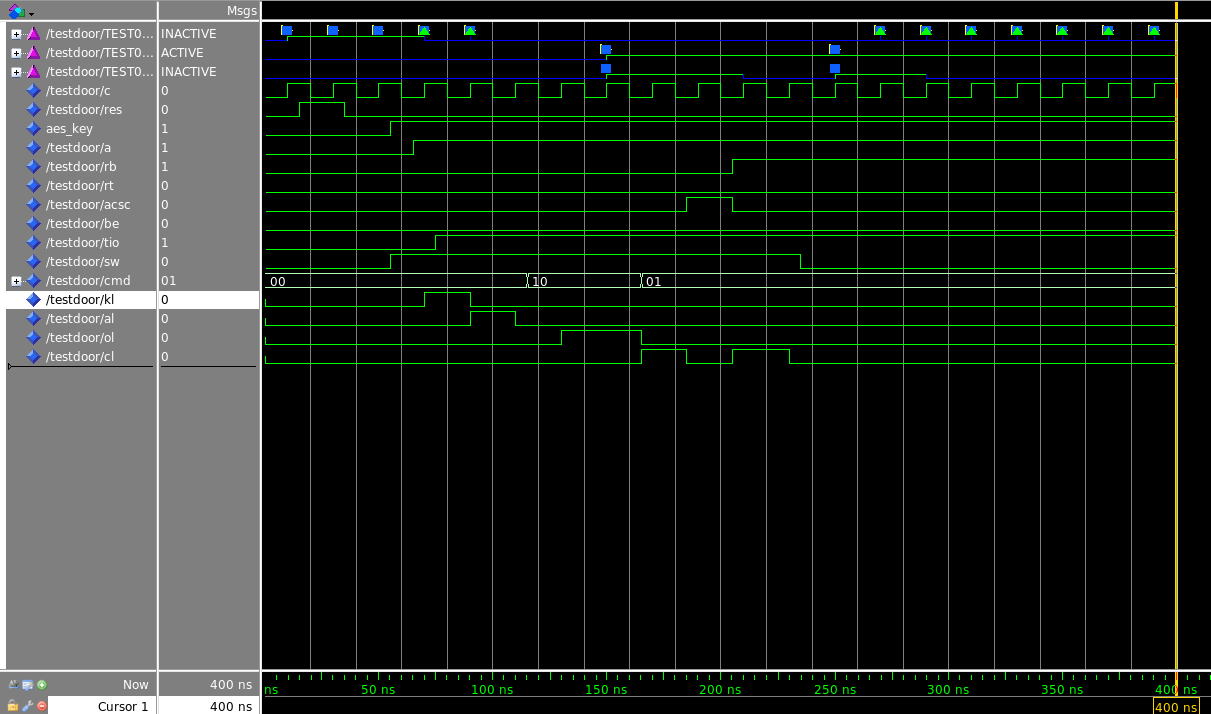
\includegraphics[width=0.9\linewidth]{PSL1assertion_model_SafetyError.png}  
      \caption{Wave form of simulating the Safety Error test bench and verifying \texttt{PSL} assertion \textit{key\_req}}
    \end{figure}
    
    \subsubsection{Open light}
    We test the second \texttt{PSL} assertion \textit{open\_l} using the Door Up test bench. The Door Up models a scenario where the system is turned on, no action occurs from the user for a short while and the system is turned off again. The \textit{open\_l} assertion specifies that when the state \textit{Down} is reached, the open light turns on only when the \textit{d\_open} command is sent/maintained without bad encryption. This assertion lasts until the door is fully open. The waveform below shows that this assertion (second one out of the three that appear at the top) is validated. The \textit{d\_open} command is received at \texttt{130ns}, whilst in state \textit{Down}. The conditions for the assertion are satisfied and thus a blue square appears on the next clock rising edge, \texttt{150ns}. Subsequently a green triangle appears on the next clock rising edge, \texttt{190ns}, after the state \textit{Up} has been reached showing that the assertion has passed.
    
    \begin{figure}[H]
      \centering
      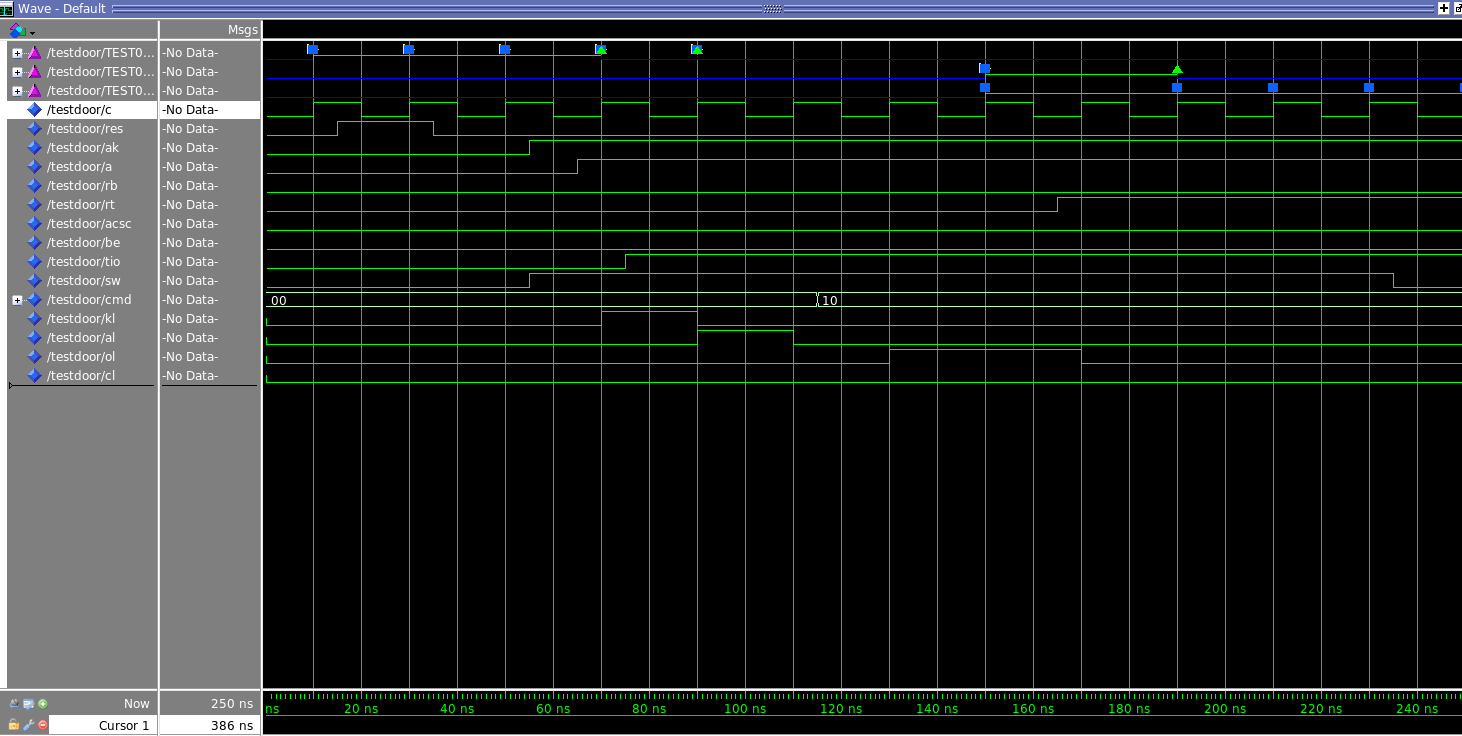
\includegraphics[width=0.9\linewidth]{PSL2assertion_model_DoorUp.png}  
      \caption{Wave form of simulating the Door Up test bench and verifying \texttt{PSL} assertion \textit{open\_l}}
    \end{figure}
    
    \subsubsection{Bad encryption}
    We test the third \texttt{PSL} assertion \textit{bad\_encryption} using the Security Error test bench. This assertion specifies that when a \textit{bad\_encryption} signal is received after the user entered either a \textit{d\_open} or \textit{d\_close} command followed by any inputs (except those that would produce errors) in state \textit{Down} or \textit{Up}, the state \textit{Security Error} is reached before eventually reaching the state \textit{Deactivated}.  The waveform below shows that this assertion (third one out of the three that appear at the top) is validated. The \textit{d\_close} command is received at \texttt{75ns}, when in state \textit{Up}. On the next clock rising edge, \texttt{90ns}, the blue square appears indicating that the assertion has begun being evaluated. Subsequently a green triangle appears at \texttt{190ns} showing that the assertion has passed.
    
    \begin{figure}[H]
      \centering
      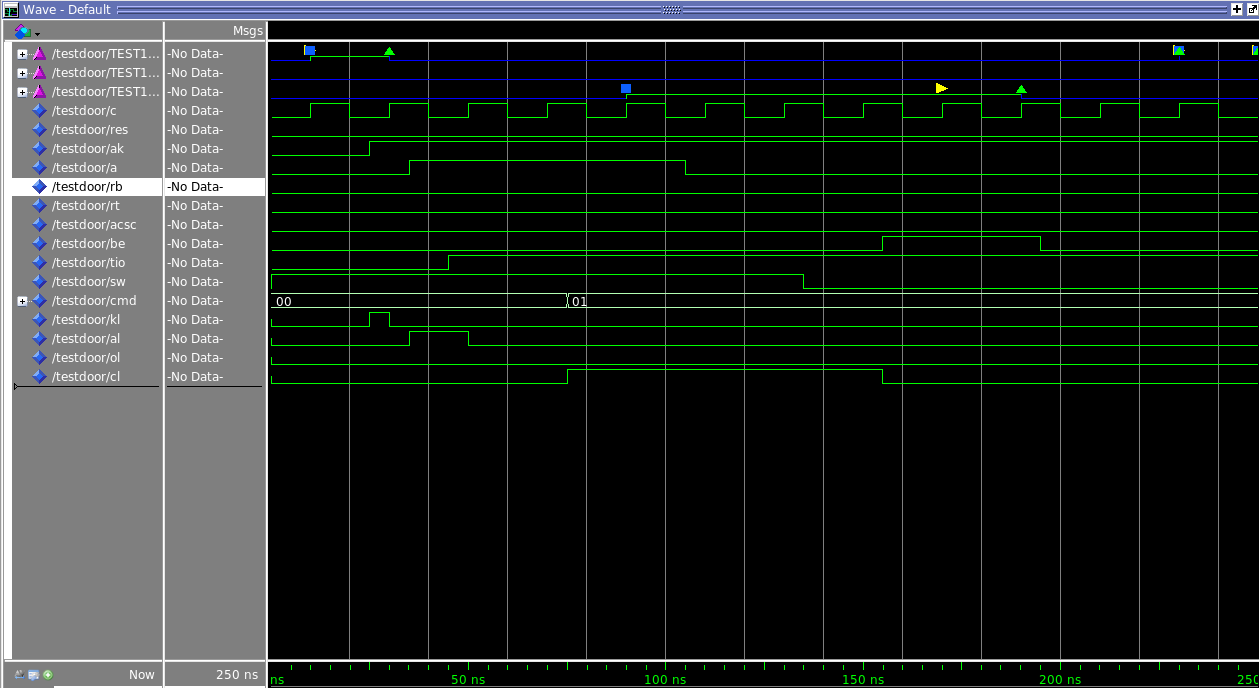
\includegraphics[width=0.9\linewidth]{PSL3_model_testSecurityError.png}  
      \caption{Wave form of simulating the Security Error test bench and verifying \texttt{PSL} assertion \textit{bad\_encryption}}
    \end{figure}
	
	\section{\texttt{ASIC} Synthesis}
	\subsection{Different Encodings}
		
	\par We performed \texttt{ASIC} synthesis with three different encodings: \texttt{One Hot}, \texttt{Gray} and \texttt{Binary}. The reports of the generated components can be found below.
	
	\par With \texttt{One-Hot} encoding, each bit of state is stored in a separate flip-flop, therefore it requires more flip-flops than binary encoding. However, with one-hot encoding, the next state and the logic function encoded by the circuit is often simpler, so fewer gates are required. With \texttt{One Hot} encoding, as expected, we obtain the largest area of \texttt{6861um2}, the shortest critical path of length \texttt{1.44} and therefore the best frequency of \texttt{691.7MHz}. As expected, we generated 11 flip-flops, the largest number compared to the other encodings.

	\par With \texttt{Gray} encoding, only one bit changes from each number to the next. In order to utilize this property, it is possible to intentionally order our state encoding according to the states traversed in our specific scenario (set up the Gray encoding according to the higher-probability path). We can use Gray encoding to reduce the power consumption of the \texttt{ASIC} component. However, we kept the same order as for the other encodings. After synthesis, we obtain a critical path length of \texttt{3.01} and a frequency of \texttt{331.8MHz}, we also observe the smallest area of \texttt{5496um2} which suggests that the synthesized component is less complex. As expected, we observe 4 flip-flops, the same number as with the binary encoding.

	\par With \texttt{Binary} encoding, the total area is in between those obtained with other encodings – \texttt{6770um2}. The critical path length is \texttt{2.59}, higher than with one-hot, and the frequency is \texttt{385.9 MHz}.
	
	\par Since we have a very small component, we are able to test all possible encodings with different orderings of states. However, it seems like this approach would not work in practice with large circuits and many components. The best encoding highly depends on the component description and needs to be chosen based on the metric that one wants to optimize (area, frequency, energy consumption).
	
\subsubsection{One Hot encoding}
\begin{minted}[mathescape]{vhdl}
 Cell      Library  References     Total Area

AOI211     c35_CORELIB     4 x     73    291 um2
AOI221     c35_CORELIB     2 x     91    182 um2
AOI311     c35_CORELIB     6 x     91    546 um2
CLKIN1     c35_CORELIB    15 x     36    546 um2
DFC1       c35_CORELIB    10 x    309   3094 um2
DFP1       c35_CORELIB     1 x    309    309 um2
NAND21     c35_CORELIB     4 x     55    218 um2
NAND31     c35_CORELIB     3 x     73    218 um2
NOR21      c35_CORELIB     6 x     55    328 um2
NOR31      c35_CORELIB     5 x     73    364 um2
NOR40      c35_CORELIB     2 x     73    146 um2
OAI211     c35_CORELIB     6 x     73    437 um2
OAI2111    c35_CORELIB     1 x     91     91 um2
OAI311     c35_CORELIB     1 x     91     91 um2

 Number of ports :                      16
 Number of nets :                       80
 Number of instances :                  66
 Number of references to this view :     0

Total accumulated area : 
 Number of um2 :                      6861
 Number of accumulated instances :      66
 
                         Clock Frequency Report

	Clock                : Frequency
      ------------------------------------

	clk                  : 691.7 MHz


                        Critical Path Report

Critical path #1, (unconstrained path)
NAME                                         GATE              ARRIVAL              LOAD
----------------------------------------------------------------------------------------
clock information not specified
delay thru clock network                                       0.00 (ideal)


reg_state(8)/QN                              DFC1        0.00  0.83 up             0.02
ix221/Q                                      NOR40       0.29  1.12 dn             0.01
ix1608/Q                                     AOI311      0.24  1.36 up             0.01
ix225/Q                                      OAI211      0.08  1.44 dn             0.01
reg_state(10)/D                              DFC1        0.00  1.44 dn             0.00
data arrival time                                              1.44


data required time                                          not specified
----------------------------------------------------------------------------------------
data required time                                          not specified
data arrival time                                              1.44
                                                            ----------
                                                         unconstrained path
----------------------------------------------------------------------------------------
\end{minted}
	
\subsubsection{Gray encoding}
\begin{minted}[mathescape]{vhdl}
 Cell      Library  References     Total Area

AOI211     c35_CORELIB     7 x     73    510 um2
AOI2111    c35_CORELIB     1 x     91     91 um2
AOI221     c35_CORELIB     1 x     91     91 um2
AOI311     c35_CORELIB     2 x     91    182 um2
CLKIN1     c35_CORELIB    15 x     36    546 um2
DFC1       c35_CORELIB     4 x    309   1238 um2
NAND21     c35_CORELIB     8 x     55    437 um2
NAND41     c35_CORELIB     2 x     91    182 um2
NOR21      c35_CORELIB     5 x     55    273 um2
NOR31      c35_CORELIB     2 x     73    146 um2
NOR40      c35_CORELIB    12 x     73    874 um2
OAI211     c35_CORELIB     4 x     73    291 um2
OAI2111    c35_CORELIB     6 x     91    546 um2
OAI221     c35_CORELIB     1 x     91     91 um2

 Number of ports :                      16
 Number of nets :                       86
 Number of instances :                  70
 Number of references to this view :     0

Total accumulated area : 
 Number of um2 :                      5496
 Number of accumulated instances :      70

                        Clock Frequency Report

	Clock                : Frequency
      ------------------------------------

	clk                  : 331.8 MHz


                        Critical Path Report

Critical path #1, (unconstrained path)
NAME                                         GATE              ARRIVAL              LOAD
----------------------------------------------------------------------------------------
clock information not specified
delay thru clock network                                       0.00 (ideal)


reg_state(2)/QN                              DFC1        0.00  0.93 up             0.04
ix149/Q                                      NOR21       0.19  1.12 dn             0.03
ix876/Q                                      NAND21      0.31  1.44 up             0.03
ix151/Q                                      CLKIN1      0.16  1.60 dn             0.02
ix921/Q                                      AOI221      0.19  1.79 up             0.01
ix163/Q                                      NOR40       0.33  2.12 dn             0.01
ix898/Q                                      AOI2111     0.26  2.38 up             0.02
ix938/Q                                      NAND41      0.07  2.45 dn             0.01
ix221/Q                                      OAI211      0.18  2.63 up             0.01
ix931/Q                                      AOI311      0.09  2.72 dn             0.01
ix273/Q                                      OAI2111     0.29  3.01 up             0.01
reg_state(3)/D                               DFC1        0.00  3.01 up             0.00
data arrival time                                              3.01


data required time                                          not specified
----------------------------------------------------------------------------------------
data required time                                          not specified
data arrival time                                              3.01
                                                            ----------
                                                         unconstrained path
----------------------------------------------------------------------------------------
\end{minted}

\subsubsection{Binary encoding}
\begin{minted}[mathescape]{vhdl}
 Cell      Library  References     Total Area

AOI211     c35_CORELIB     1 x     73     73 um2
AOI221     c35_CORELIB     2 x     91    182 um2
AOI311     c35_CORELIB     6 x     91    546 um2
CLKIN1     c35_CORELIB    19 x     36    692 um2
DFC1       c35_CORELIB     4 x    309   1238 um2
NAND21     c35_CORELIB    12 x     55    655 um2
NAND31     c35_CORELIB     2 x     73    146 um2
NAND41     c35_CORELIB     3 x     91    273 um2
NOR21      c35_CORELIB     7 x     55    382 um2
NOR31      c35_CORELIB     1 x     73     73 um2
NOR40      c35_CORELIB    14 x     73   1019 um2
OAI211     c35_CORELIB     8 x     73    582 um2
OAI2111    c35_CORELIB     3 x     91    273 um2
OAI221     c35_CORELIB     3 x     91    273 um2
OAI311     c35_CORELIB     4 x     91    364 um2

 Number of ports :                      16
 Number of nets :                      105
 Number of instances :                  89
 Number of references to this view :     0

Total accumulated area : 
 Number of um2 :                      6770
 Number of accumulated instances :      89
                         Clock Frequency Report

	Clock                : Frequency
      ------------------------------------

	clk                  : 385.9 MHz


                        Critical Path Report

Critical path #1, (unconstrained path)
NAME                                         GATE              ARRIVAL              LOAD
----------------------------------------------------------------------------------------
clock information not specified
delay thru clock network                                       0.00 (ideal)


reg_state(1)/QN                              DFC1        0.00  1.12 up             0.08
ix117/Q                                      NOR40       0.49  1.61 dn             0.04
ix924/Q                                      NAND31      0.30  1.91 up             0.01
ix123/Q                                      OAI311      0.13  2.04 dn             0.01
ix917/Q                                      AOI311      0.21  2.26 up             0.01
ix175/Q                                      OAI2111     0.09  2.35 dn             0.01
ix877/Q                                      NOR40       0.15  2.50 up             0.01
ix221/Q                                      CLKIN1      0.09  2.59 dn             0.01
reg_state(0)/D                               DFC1        0.00  2.59 dn             0.00
data arrival time                                              2.59


data required time                                          not specified
----------------------------------------------------------------------------------------
data required time                                          not specified
data arrival time                                              2.59
                                                            ----------
                                                         unconstrained path
----------------------------------------------------------------------------------------
\end{minted}
	
	\subsection{Modified temporal assertions}

    \par After \texttt{ASIC} synthesis, if one wants to make sure that the synthesis was successful a good idea is to run the same tests and validate the same temporal assertions on the synthesized component. However, it is necessary to adapt the assertions depending on the chosen encoding. Here, as an example, we include the modified assertions for binary encoding.	We first give the definition of the enumerated \textit{State} type that specifies the order in which the states will be encoded.
	\begin{minted}[mathescape]{vhdl}
    type States is (PowerUp, PowerDown, NoKey, Deactivated, Activated, Up, Down,
	SecurityError, SafetyError, MovingOnUp, MovingOnDown);
	\end{minted}
	The modified temporal assertions to be verified with \texttt{ASIC} component where states are encoded in binary:
	\begin{minted}[mathescape]{vhdl}
    -- Implication should be true at the same time as the condition is true.
    PSL property key_req is always (((state_0 = '0' and state_1 = '0' and state_2 = '0'
    and state_3 = '0') or (state_0 = '0' and state_1 = '0' and state_2 = '0' and state_3 = '1'))
    -> (state_0 /= '0' and state_1 /= '1' and state_2 /= '0' and state_3 /= '0')
    until (aes_key = '1'));

    -- Implication should be true at the same time as the condition is true.
    PSL property open_l is always ((state_0 = '0' and state_1 = '1' and state_2 = '1'
    and state_3 = '0') -> ((open_light = '1') ->
    (command = "10" and bad_encryption = '0' and acsc = '0'))
    until (state_0 = '0' and state_1 = '1' and state_2 = '0' and state_3 = '1'));

    -- Suffix implication should be true at the next clock cycle after the left r. exp.
    has been recognized.
    PSL property bad_enc is always ({((state_0 = '0' and state_1 = '1' and state_2 = '1'
    and state_3 = '0') or (state_0 = '0' and state_1 = '1' and state_2 = '0' and state_3 = '1'));
    ((command = "01" or command = "10") and (bad_encryption = '0'));
    (bad_encryption = '1' nor acsc = '1')[*]; bad_encryption = '1'}
    |-> (state_0 = '0' and state_1 = '1' and state_2 = '1' and state_3 = '1')
    before (state_0 = '0' and state_1 = '0' and state_2 = '1' and state_3 = '1'));
	\end{minted}

	\subsection{Simulation after synthesis}
	\par We can inspect the synthesized \texttt{ASIC} component with one-hot encoding in visual form.

	\begin{figure}[H]
	    \centering
	    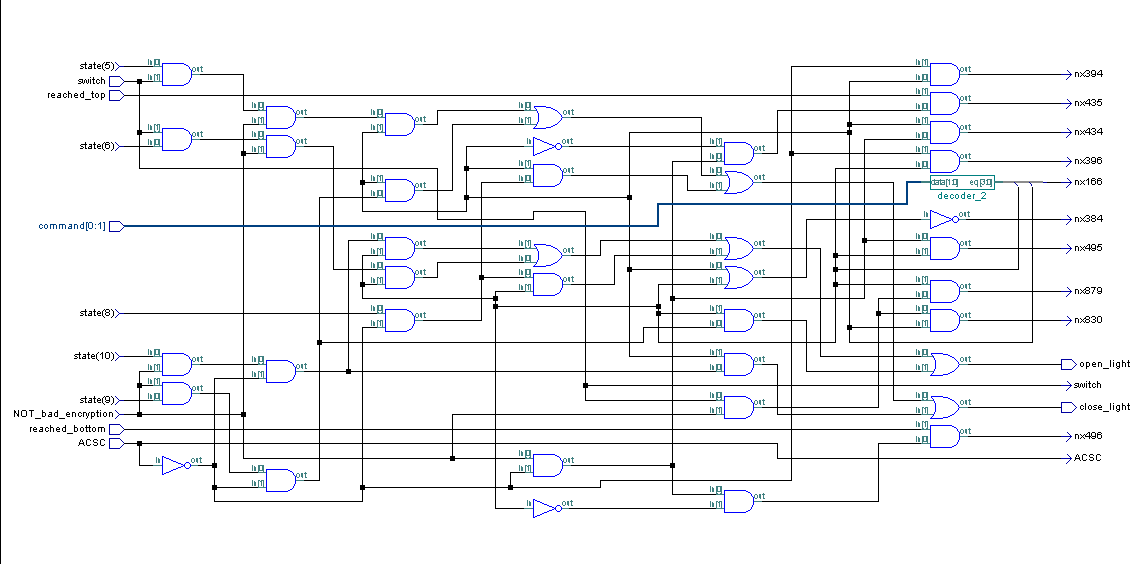
\includegraphics[width=0.8\linewidth]{OneHotASIC.png}
	    \caption{Synthesized \texttt{ASIC} component with one-hot encoding}
	\end{figure}
	
	\par For simulation we use the synthesized component with binary encoding according to the order in the $State$ type definition given earlier. In the waveform of the Safety Error test bench simulation the states (four flip-flops) are changing as expected and produce the same outputs as the finite state machine model simulation discussed in $2.1$.
	\begin{figure}[H]
	    \centering
	    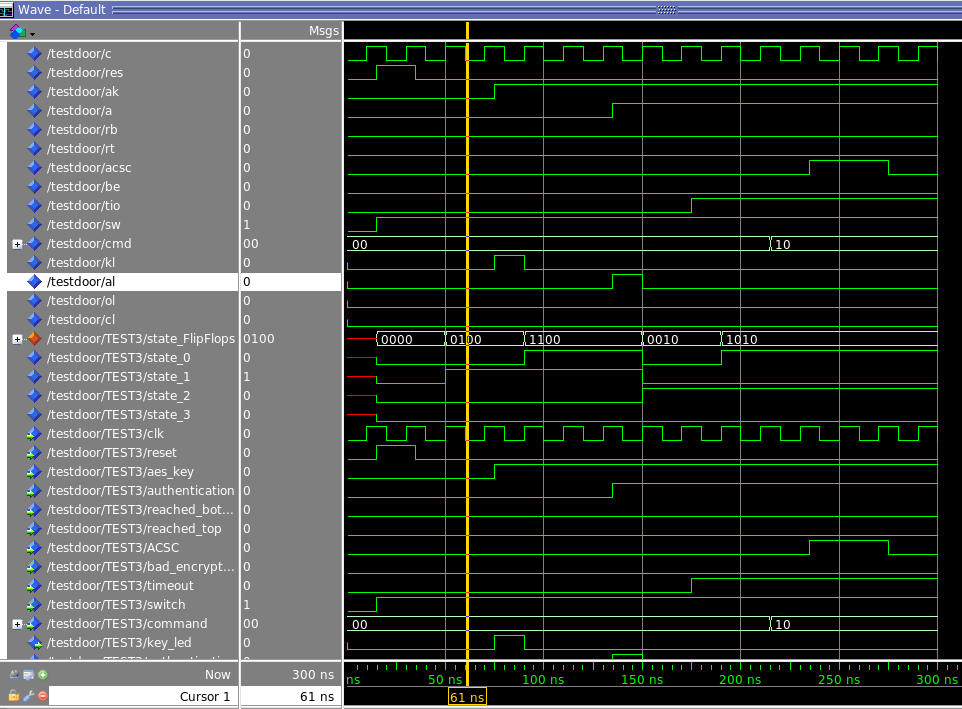
\includegraphics[width=1\linewidth]{Synthesized.png}
	    \caption{Waveform of Safety Error test bench on a synthesized \texttt{ASIC} component with binary encoding}
	\end{figure}

	\section{\texttt{FPGA} synthesis}
	
	\par Before performing \texttt{FPGA} synthesis on an \texttt{Altera Cyclone II DE1} board we modify our \texttt{VHDL} description to match the default clock of the board, visualize the outputs on the provided LED screen, map the output of the \texttt{FPGA} onto the LED's of the board and map the toggle switch inputs of the board to the inputs of the \texttt{FPGA} .
	
	\subsection{Synthesis report}
	\par After having made the necessary modifications to the \texttt{VHDL} description of our component and performing \texttt{FPGA} synthesis on an \texttt{Altera Cyclone II DE1} board, we notice that we only use less than \texttt{1\%} of the area of the entire \texttt{FPGA} . This is because we have a very small component. In real life applications a larger percentage of the \texttt{FPGA} would be used. We have 37 registers, which is large considering that we only have 11 states, however this is the result of having to reconfigure the clock to match the default clock of the \texttt{Altera Cyclone II DE1}. 
	\begin{figure}[H]
	    \centering
	    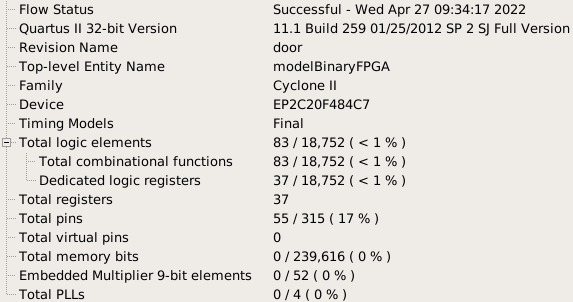
\includegraphics[width=0.5\linewidth]{PROJECT2.png}
	    \caption{\texttt{FPGA} synthesis report}
	\end{figure}
	
	\subsection{Visualizing the component}
	\par In the visual representation of the synthesized \texttt{FPGA} we can identify some clear differences with the \texttt{ASIC} component. We notice that instead of having custom gates that are optimized and specific to the \texttt{VHDL} description, we obtain a mapping from our finite state machine to the existing wires, gates and memory components of the \texttt{FPGA} .
	\begin{figure}[H]
	    \centering
	    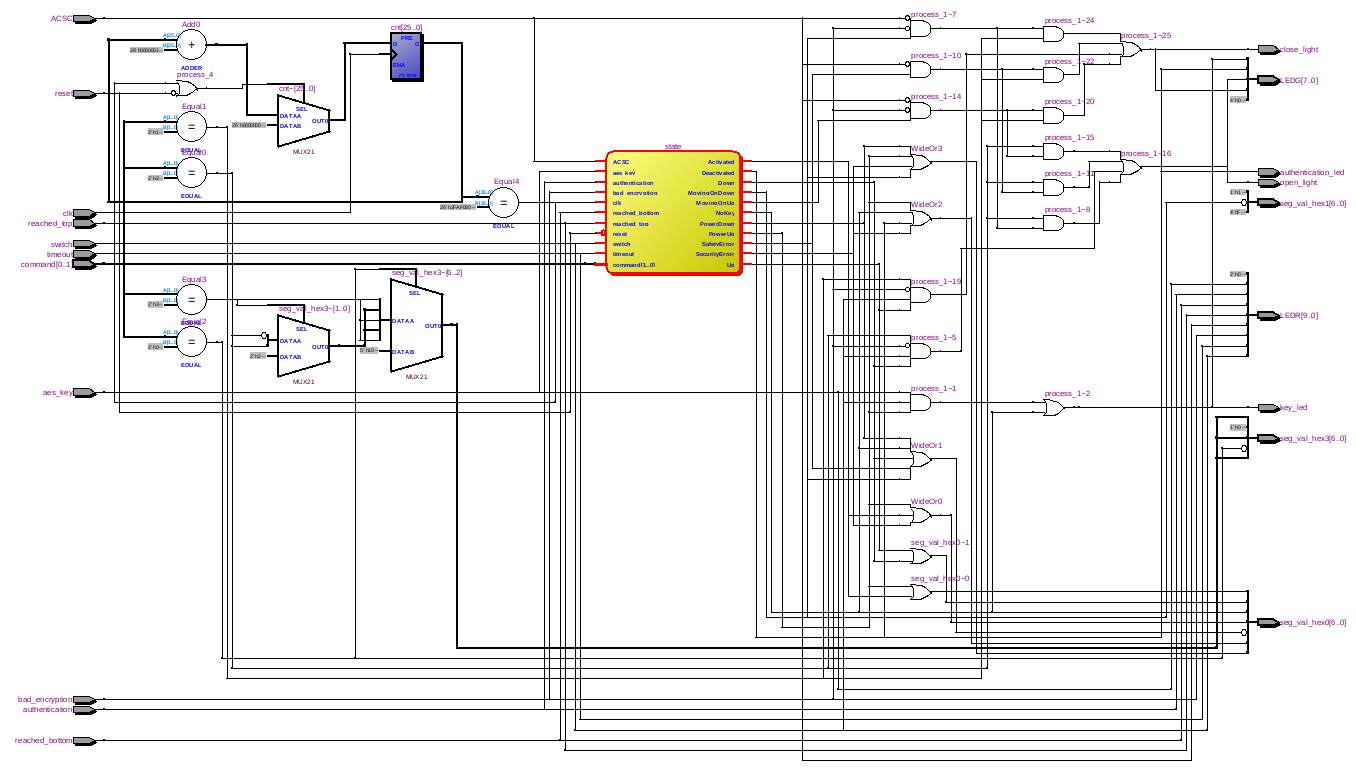
\includegraphics[width=0.9\linewidth]{PROJECT1.png}
	    \caption{Caption}
	    \caption{Synthesized \texttt{FPGA} component}
	\end{figure}

	\section{Conclusion}
	
	\par This project allowed us to observe the design process of a circuit component, from an incomplete textual description to synthesis.
	\par Besides learning how to specify components and create their architecture, we saw techniques to validate a component description. We were able to write test benches for multiple scenarios, see how to check how much of the system our tests cover and assert some temporal statements that need to be verified. These techniques allowed us to detect bugs and improve our description before performing synthesis.
	\par After synthesizing an \texttt{ASIC} circuit we could observe the relationship between a high-level behavioural description of a circuit and its physical hardware representation. By identifying the number of memory elements synthesized we were able to fix any remaining bugs in our \texttt{VHDL} description. In this stage we identified differences between various encodings. We concluded that these encodings offer different benefits and it is important to select an appropriate encoding in order to maximize performance according to one's metrics.
	\par After performing two types of synthesis, we observed some notable differences between \texttt{ASIC} and \texttt{FPGA}. The \texttt{ASIC} component seemed more optimized for our garage controller. Also, since our circuit is very small, much of the available \texttt{FPGA} was not utilized. However, in a real world scenario it might still be cheaper and easier to customize an \texttt{FPGA} rather than producing a custom \texttt{ASIC} for a garage door controller, especially considering that the implemented controller would only be a small part of the whole system.
	\par This project gave us a glimpse into the process of designing and testing hardware components. It showed us that besides rigorous logic and satisfiability considerations, one must take into account real-world scenarios and decide which trade-offs to make depending on the budget, time or other constraints.

    \newpage
    \section{Appendix}
    
    \begin{minted}[mathescape]{vhdl}
    -- Safety Error test banch used for waveform simulation in section 2.1
        generic map(init_closed => True)
        -- Creating the port map.
        port map(c, res, ak, a, rb, rt, acsc, be, tio, sw, cmd, kl, al, ol, cl);
        -- Simulation scenario where the door opens, then a safety error occurs
        -- while it's being closed.
        res <= '1' after 15 ns, '0' after 35 ns;
        sw <= '1' after 55 ns, '0' after 235 ns;
        ak <= '1' after 55 ns;
        a <= '1' after 65 ns;
        tio <= '1' after 75 ns;
        cmd <= "10" after 115 ns, "01" after 165 ns;
        acsc <= '1' after 185 ns, '0' after 205 ns;
        rb <= '1' after 205 ns;
        -- 50 MHz clock
        c <= not(c) after 10 ns;
        ------------------------------------------------------
    -- Safety Error test banch used for temporal assertions in section 3.1.1
        generic map(init_closed => True)
        -- Creating the port map.
        port map(c, res, ak, a, rb, rt, acsc, be, tio, sw, cmd, kl, al, ol, cl);
        -- Simulation scenario where the door opens, then a safety error occurs
        -- while it's being closed.
        sw <= '1' after 15 ns, '0' after 195 ns;
        ak <= '1' after 15 ns;
        a <= '1' after 25 ns;
        tio <= '1' after 35 ns;
        cmd <= "10" after 65 ns, "01" after 125 ns;
        acsc <= '1' after 145 ns, '0' after 165 ns;
        rb <= '1' after 165 ns;
        -- 50 MHz clock
        c <= not(c) after 10 ns;
    \end{minted}
    
    \begin{minted}[mathescape]{vhdl}
    -- Security Error Test Bench used for simulation in section 2.2
        generic map(init_closed => False)
        -- Creating the port map.
        port map(c, res, ak, a, rb, rt, acsc, be, tio, sw, cmd, kl, al, ol, cl);
        -- Second simulation scenario where the initially open door is
        -- being closed and a security error occurs.
        sw <= '1' after 0 ns, '0' after 135 ns;
        ak <= '1' after 25 ns;
        a <= '1' after 35 ns, '0' after 105 ns;
        tio <= '1' after 45 ns;
        cmd <= "01" after 75 ns;
        be <= '1' after 155 ns, '0' after 195 ns;
        -- 50 MHz clock
        c <= not(c) after 10 ns;
        ------------------------------------------------------
    -- Security Error Test Bench used for temporal assertions in section 3.1.2
        sw <= '1' after 0 ns, '0' after 135 ns;
        ak <= '1' after 25 ns;
        a <= '1' after 35 ns;
        tio <= '1' after 45 ns;
        cmd <= "01" after 75 ns;
        be <= '1' after 105 ns, '0' after 135 ns;
        -- 50 MHz clock
        c <= not(c) after 10 ns;
    \end{minted}
    
    \begin{minted}[mathescape]{vhdl}
    -- Door Up Test Bench used for temporal assertions in section 3.1.3
        generic map(init_closed => True)
        -- Creating the port map.
        port map(c, res, ak, a, rb, rt, acsc, be, tio, sw, cmd, kl, al, ol, cl);
        -- Simulation scenario where the door fully opens.
        res <= '1' after 15 ns, '0' after 35 ns;
        sw <= '1' after 55 ns, '0' after 235 ns;
        ak <= '1' after 55 ns;
        a <= '1' after 65 ns;
        tio <= '1' after 75 ns;
        cmd <= "10" after 115 ns;
        rt <= '1' after 165 ns;
        -- 50 MHz clock
        c <= not(c) after 10 ns;
    \end{minted}
    
    \begin{minted}[mathescape]{vhdl}
    -- Architecture of the garage door controller as a Mealy machine
        library IEEE;
        use IEEE.std_logic_1164.all;
        -- Input and output ports of the garage door controller.
        entity door is
        generic (init_closed : boolean := False);
        port(
            -- Input ports.
            clk, reset, aes_key, authentication, reached_bottom, reached_top, ACSC,
            bad_encryption, timeout, switch: in std_logic;
            command: in std_logic_vector(0 to 1);
	    -- Output ports.
	    key_led, authentication_led, open_light, close_light: out std_logic);
        end door;

        architecture Automaton of door is
            -- States of the finite state machine.
            type States is (PowerUp, PowerDown, NoKey, Deactivated, Activated, Up, Down,
            SecurityError, SafetyError, MovingOnUp, MovingOnDown);
            -- Inner signals.
            signal state, next_state: States;
        
            -- PSL default clock is (clk'event and clk = '1');

            -- Being in states PowerUp or PowerDown implies that the current state is not
            -- Activated until aes_key is on.
            -- PSL property key_req is always ((state = PowerUp or state = PowerDown) ->
            -- (state /= Activated) until (aes_key = '1'));

            -- Being in state Down implies that open_light turns on only when the open_door
            -- command is sent  without bad encryption nor acsc signal until the door is open.
            -- PSL property open_l is always ((state = Down) -> ((open_light = '1') ->
            -- (command = "10" and bad_encryption = '0' and acsc = '0')) until (state = Up));

            -- If state is Down or Up, then command is open or close and bad encryption is false.
            -- PSL property bad_enc is always ({(state = Down or state = Up); ((command = "01" or
            -- command = "10") and (bad_encryption = '0')); (bad_encryption = '1' nor
            -- acsc = '1')[*]; bad_encryption = '1'} |-> (state = SecurityError) before
            -- (state = Deactivated));

            -- PSL assert key_req;
            -- PSL assert open_l;
            -- PSL assert bad_enc;

            begin
            -- Transition function of the finite state machine of the garage door controller.
            process(state, aes_key, authentication, reached_bottom, reached_top, ACSC,
            bad_encryption, timeout, switch, command)
                begin
                    case state is
                        -- All transitions from the state PowerUp.
                        when PowerUp =>
                            if (switch = '0') then next_state <= PowerDown;
                            else
                                if (aes_key = '0') then next_state <= NoKey;
                                else next_state <= Deactivated;
	                            end if;
	                        end if;
                        -- All transitions from the state PowerDown.
                        when PowerDown =>
                            if (switch = '0') then next_state <= PowerDown;
                            else
                                next_state <= PowerUp;
	                        end if;
                        -- All transitions from the state NoKey.
                        when NoKey =>
                            if (switch = '0') then next_state <= PowerDown;
                            else
                                if (aes_key = '0') then next_state <= NoKey;
                                else next_state <= Deactivated;
	                            end if;
	                        end if;
                        -- All transitions from the state Deactivated.
                        when Deactivated =>
                            if (switch = '0')
                                then next_state <= PowerDown;
                            else
                                if (authentication = '0') then next_state <= Deactivated;
                                else next_state <= Activated;
	                            end if;
	                        end if;
                        -- All transitions from the state Activated.
                        when Activated =>
                            if (command = "11") then next_state <= Deactivated;
                            else
                                if (timeout = '1') then
                                    if (init_closed) then next_state <= Down;
			                        else next_state <= Up;
	                                end if;
                                else next_state <= Activated;
	                            end if;
	                        end if;
                        -- All transitions from the state Up.
                        when Up =>
                            if (switch = '0')
                                then next_state <= PowerDown;
                            elsif (switch = '1' and bad_encryption = '1')
                                then next_state <= SecurityError;
                            elsif (switch = '1' and bad_encryption = '0' and command = "01")
                                then next_state <= MovingOnDown;
                            else next_state <= Up;
	                        end if;
                        -- All transitions from the state Down.
                        when Down =>
                            if (switch = '0')
                                then next_state <= PowerDown;
                            elsif (switch = '1' and bad_encryption = '1')
                                then next_state <= SecurityError;
                            elsif (switch = '1' and bad_encryption = '0' and command = "10")
                                then next_state <= MovingOnUp;
                            else next_state <= Down;
	                        end if;
                        -- All transitions from the state SecurityError.
                        when SecurityError => next_state <= Deactivated;
                        -- All transitions from the state SafetyError.
                        when SafetyError =>
                            if (ACSC = '0') then
                                if (command = "01")
                                    then next_state <= MovingOnDown;
                                elsif (command = "10")
                                    then next_state <= MovingOnUp;
			                    else next_state <= SafetyError;
	                            end if;
                            else next_state <= SafetyError;
	                        end if;
                        -- All transitions from the state MovingOnUp.
                        when MovingOnUp =>
                            if (bad_encryption = '1')
                                then next_state <= SecurityError;
                            elsif (bad_encryption = '0' and ACSC = '1')
                                then next_state <= SafetyError;
                            elsif (bad_encryption = '0' and ACSC = '0' and command = "01")
                                then next_state <= MovingOnDown;
                            elsif (bad_encryption = '0' and ACSC = '0' and command /= "01" and
                                   reached_top = '1')
                                then next_state <= Up;
                            else next_state <= MovingOnUp;
	                        end if;
                        -- All transitions from the state MovingOnDown.
                        when MovingOnDown =>
                            if (bad_encryption = '1')
                                then next_state <= SecurityError;
                            elsif (bad_encryption = '0' and ACSC = '1')
                                then next_state <= SafetyError;
                            elsif (bad_encryption = '0' and ACSC = '0' and command = "10")
                                then next_state <= MovingOnUp;
                            elsif (bad_encryption = '0' and ACSC = '0' and command /= "10" and
                                   reached_bottom = '1')
                                then next_state <= Down;
                            else next_state <= MovingOnDown;
	                        end if;
                end case;
            end process;

            -- Output function.
            process(state, aes_key, authentication, reached_bottom, reached_top, ACSC,
            bad_encryption, timeout, switch, command)
                begin
                    -- Initially setting everything to zero.
                    key_led <= '0';
                    authentication_led <= '0';
                    open_light <= '0';
                    close_light <= '0';
                    -- Setting the key_led output.
                    if ((state = PowerUp and switch = '1' and aes_key = '1')
                    or  (state = NoKey and switch = '1' and aes_key = '1'))
                        then key_led <= '1';
	                end if;
                    -- Setting the authentication_led output.
                    if (state = Deactivated and switch = '1' and authentication = '1')
                        then authentication_led <= '1';
	                end if;
                    -- Setting the open_light output.
                    if ((state = Down and switch = '1' and bad_encryption = '0'
                        and command = "10")
                    or  (state = MovingOnDown and bad_encryption = '0' and ACSC = '0'
                        and command = "10")
                    or  (state = SafetyError and ACSC = '0' and command = "10")
                    or  (state = MovingOnUp and bad_encryption = '0' and ACSC = '0'
                        and command = "10"))
                        then open_light <= '1';
	                end if;
                    -- Setting the close_light output.
                    if ((state = Up and switch = '1' and bad_encryption = '0'
                        and command = "01")
                    or  (state = MovingOnUp and bad_encryption = '0' and ACSC = '0'
                        and command = "01")
                    or  (state = SafetyError and ACSC = '0' and command = "01")
                    or  (state = MovingOnDown and bad_encryption = '0' and ACSC = '0'
                        and command = "01"))
                        then close_light <= '1';
	                end if;
            end process;

            -- Updating of the state register on the clock rising edge.
            process(reset, clk)
                begin
                    if (reset='1') then state <= PowerUp;
                    elsif (clk'event and clk='1') then state <= next_state;
	                end if;
            end process;
        end Automaton;
    \end{minted}
    
\end{document}
